\documentclass[12pt,a4paper]{article}

\usepackage[letterpaper]{geometry}

\usepackage{times}
\geometry{top=1.0in, bottom=1.5in, left=1.0in, right=1.0in}

\usepackage{fancyhdr}
\pagestyle{fancy}
\lhead{}
\rhead{}
\lfoot{}
\rfoot{}

\renewcommand{\headrulewidth}{0pt} 
\renewcommand{\footrulewidth}{0pt} 

\setlength\headsep{0.333in}

\usepackage{fontspec}
%\setmainfont{Times New Roman}

\usepackage{graphicx}

\usepackage{hyperref}

\usepackage{caption}

\usepackage{indentfirst}

\usepackage{setspace}

\usepackage{float}

\usepackage{enumitem}
\usepackage{listings}
\usepackage{color}
\usepackage{xcolor}

\usepackage{tabularx}

\usepackage{amsmath}

\begin{document}

\begin{titlepage}
\begin{center}
\vspace*{2cm}

\doublespacing
\rule{\linewidth}{0.3mm}

\textsc{
	\large
	UM-SJTU Joint Institute\\ 
	Physical Laboratory\\
	VP141
}

\rule{\linewidth}{0.3mm}


\vspace*{3.5cm}

{
\Large
\textsc{Laboratory Report}\\
}

\vspace*{0.2cm}

{
\large
\textsc{Exercise 1} \\
\textsc{Measurements of the Moment of Inertia}
}

\end{center}

\vfill
\normalsize

\hspace*{1cm}
\begin{minipage}{0.4\textwidth}
\begin{tabular}{p{1.7cm}p{4cm}llll}
Name: &  Ren Wang \hspace*{0.5cm} {\fontspec{Hei}\selectfont 王韧} & ID: & 516370910177 & Group: & 11 \\
\multicolumn{6}{l}{Date: \today}
\end{tabular}
\end{minipage}

\end{titlepage}

%\setmainfont{Times New Roman}
\doublespacing 
\newpage

\section{Theoretical Background}

Moment of inertia of a rigid body about an axis is a quantitative
characteristics that defines the body’s resistance (inertia) to a change of
angular velocity in rotation about that axis. 
This characteristics of the rigid body rotating about a fixed axis is determined
not only by the mass of the body, but also by its distribution. 
The moment of inertia of a rigid body about a certain rotation axis can be
calculated analytically. 
However, if the body has irregular shape or non-uniformly distributed mass, the
calculation may be di cult.
Experimental methods turn out to be more useful in such cases.

\subsection{Laws of Physics Used}

There are mainly two laws of Physics been used in the experiment. Second law of
dynamics for rotational motion can find the relationship between the rotational
acceleration and the torque at the object.

\subsubsection{Second Law of Dynamics for Rotational Motion}

The rotational motion about a fixed axis relates with the component of the
torque about the axis of rotation with the moment of inertia about this axis.
$$ \tau_z = I\beta_z$$
Therefore, the moment of inertia I can be found once the torque and the
resulting angular acceleration are measured.

The moment of inertia is an additive quantity, the moment of inertia of the
combined rigid body AB composed of A and B, about the same axis of rotation, is 
$$ I_{ab} = I_A + I_B $$


\subsubsection{Parallel Axis Theorem}
If the moment of inertia of a rigid body with mass m about an axis through the
body’s center of mass is I0, then for any axis parallel to that axis, the moment
of inertia is
$$ I = I_0 + md^2 $$
where $d$ is the distance between the axes.

\section{Apparatus}
The measurement setup consists of a turntable with an integrated photo-gate
system used for time measurements.
\singlespacing
\begin{itemize}
\item sample
\item turntable
\item photo gate holder
\item pulley
\item string
\item weight
\item photo gate
\item shielding pin
\item cone pulley
\item levelling bolt
\item arm holder
\end{itemize}
\doublespacing

\begin{figure}[H]
\centering
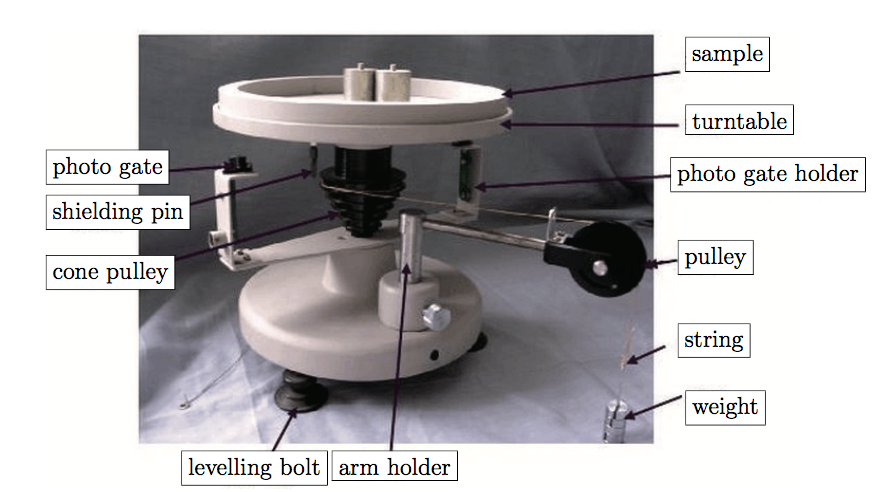
\includegraphics[width=15cm]{fig/app/turntable}
\end{figure}

Since the bearings of the turntable are not frictionless, there will be a
non-zero frictional torque $M_μ$ causing the turntable to decelerate with
angular acceleration $\beta_1$, so that the second law of dynamics for
rotational motion of the empty turntable reads $$   M_\mu = -I_1\beta_1  $$
\section{Procedure}
\begin{enumerate}
\item Measure the mass of the weight, the hoop, the disk, and the cylinder, as
  well as the radius of the cone pulley and the cylinder (follow the
  instructor’s requirements). Calculate the moment of inertia of the hoop and
  the disk analytically.
\item Turn the electronic timer on and switch it to mode 1-2 (single gate,
  multiple pulses). 
\item Place the instrument close to the edge of the desk and stretch the disk
  pulley arm outside, so that the weight can move downwards unobstructed. 
\item Level the turntable with the bubble level.
\item Make the turntable rotating and press the start button on the timer. After
  at least 8 signals are recorded, stop the turntable and record the data in
  your data sheet. 
\item Attach the weight to one end of the string. Place the string on the disk
  pulley, thread through the hole in the arm, and wind the string around the 3rd
  ring of the cone pulley. Adjust the arm holder so that the string goes through
  the center of the hole. 
\item Release the weight and start the timer. Stop the turntable when the weight
  hits the floor. Write down the recorded data. 
\item The angular acceleration can be found by plotting $\theta =k\pi$ against
  $t$ and performing a quadratic fit using data processing software. (The
  magnitude of the angular acceleration is equal to the coefficient next to
  $t^2$ multiplied by two. The uncertainty of the angular acceleration can be
  read directly from the fitting result.) 

  The moment of inertia of the empty turntable is found by using the formulae in
  Section 3 and the data from step 5 and 7. Repeat steps 5--7 with a rigid
  object placed on the turntable. An equaition is used to find the moment of
  inertia of the rigid object. 
\end{enumerate}
The timer’s resolution is $0.0001 s$, and the error is $0.004\%$. 

\section{Calculations and Results}
From the following equaitions,

$$ \tau_z = I\beta_z $$
$$ I_{ab} = I_A + I_B $$
$$ M_\mu = -I_1\beta_1 $$
$$ T = m(g-a)$$

We can derive
$$ m(g-R\beta_2)R-M_\mu=I_1\beta_2 $$
Then we find
$$ I_1=\frac{mR(g-R\beta_2)}{\beta_2-\beta_1} $$
Similarly, if a rigid body with an unknown moment of inertia is placed on the
turntable, we may find 
$$ I_2=\frac{mR(g-R\beta_4)}{\beta_4-\beta_3} $$
Using the fact that the moment of inertia is an additive quantity, the moment of
inertia of the rigid object placed on the turntable, with respect to the axis of
rotation, may be found as the difference 
$$ I_3 = I_2 - I_1 $$

\subsection{Measurement of Angular Acceleration}
Angular acceleration can be derive by investigating the measurement data (k,t),
the corresponding angular position is
$$ \theta = k\pi = \omega_0 t + \frac{1}{2}\beta t^2 $$


\subsection{In Lab Data}

\begin{table}[H]
  \centering
  \begin{tabularx}{\textwidth}{|p{6cm}|X|X|X|X|}
    \hline
    Object & 1 & 2 & 3 & 4 \\
    \hline
    Disk $[cm] \pm 0.002[cm]$& 24.098 & 24.094 & 24.094 & 24.094 \\
    Hoop 1 $[cm] \pm 0.002[cm]$& 20.982 & 20.918 & 20.966 & 20.976 \\
    Hoop 2 $[cm] \pm 0.002[cm]$& 23.998 & 24.000 & 24.000 & 24.002 \\
    Cylinder A $[cm] \pm 0.002[cm]$& 2.994 & 2.994 & 2.994 & 2.994 \\
    Cylinder B $[cm] \pm 0.002[cm]$& 2.994 & 2.994 & 2.994 & 2.994 \\
    Cone pulley $[cm] \pm 0.002[cm]$& 5.022 & 5.020 & 5.008 & 5.008 \\
    Hole 1 d $[cm] \pm 0.002[cm]$& 3.978 & 5.534 & & \\
    Hole 2 d $[cm] \pm 0.002[cm]$& 3.982 & 5.540 & & \\
    Hole 3 d $[cm] \pm 0.002[cm]$& 5.524 & 6.500 & & \\
    Hole 4 d $[cm] \pm 0.002[cm]$& 5.520 & 6.520 & & \\
    \hline
  \end{tabularx}
  \caption{Calliper measurements}
  \end{table}


\begin{table}[H]
  \centering
  \begin{tabularx}{\textwidth}{|X|X|}
    \hline
    Object & Mass\\
	\hline
    Disk $[g] \pm 0.1 [g] $ & 493.1\\
    Hoop $[g] \pm 0.1 [g] $ & 422.5\\
    Cylinder A $[g] \pm 0.1 [g] $ & 165.8\\
    Cylinder B $[g] \pm 0.1 [g] $ & 165.8\\
    Weight $[g] \pm 0.1 [g] $ & 59.1 \\
    \hline
  \end{tabularx}
  \caption{Mass measurements}
  \end{table}
% begin real data
\begin{table}[H]
  \centering
\begin{tabular}{|p{2cm}|p{1.5cm}|l|l|l|l|l|l|l|l|l|}
\hline
Situation & A or D & k & 1 & 2 & 3 & 4 & 5 & 6 & 7 & 8 \\
\hline
Empty & Dec & $t[s]$ & 0.2958 & 0.5924 & 0.8899 & 1.1881 & 1.4873 & 1.7871 & 2.0879 & 2.3895 \\
Empty & Acc & $t[s]$ & 0.9005 & 1.5186 & 2.0204 & 2.4557 & 2.8448 & 3.1996 & 3.5280 & 3.7038 \\
With disk & Dec &  $t[s]$ & 0.3178 & 0.6362 & 0.9554 & 1.2752 & 1.5958 & 1.9170 & 2.2390 & 2.5616 \\
With disk & Acc &  $t[s]$ & 0.8957 & 1.5808 & 2.1582 & 2.6666 & 3.1264 & 3.5491 & 3.9428 & 4.3322 \\
With hoop & Dec &  $t[s]$ & 0.2450 & 0.4903 & 0.7359 & 0.9818 & 1.2281 & 1.4746 & 1.7216 & 1.9688 \\
With hoop & Acc &  $t[s]$ & 1.0035 & 1.7614 & 2.3967 & 2.9547 & 3.4589 & 3.9216 & 4.3521 & 4.7560 \\
A 1 B 2 & Dec &  $t[s]$ & 0.4491 & 0.9003 & 1.3536 & 1.8089 & 2.2666 & 2.7263 & 3.1883 & 3.6524 \\
A 1 B 2 & Acc &  $t[s]$ & 1.3586 & 2.0905 & 2.6595 & 3.1424 & 3.5692 & 3.9562 & 4.3125 & 4.6448 \\
A 3 B 4 & Dec &  $t[s]$ & 0.4539 & 0.9099 & 1.3678 & 1.8279 & 2.2899 & 2.7541 & 3.2204 & 3.6888 \\
A 3 B 4 & Acc &  $t[s]$ & 1.3748 & 2.1298 & 2.7179 & 3.2171 & 3.6585 & 4.0587 & 4.4273 & 4.7711 \\
\hline
\end{tabular}
\caption{ Time measurements}
\end{table}

According to  United States Department of Commerce, the standard gravitational
acceleration is 
$$ g =  9.80665 m/s^2 $$

% ==================================================================
% ==================================================================
For the Empty turntable,
\newcommand{\EFWwr}{17cm}
\begin{figure}[H]
\centering
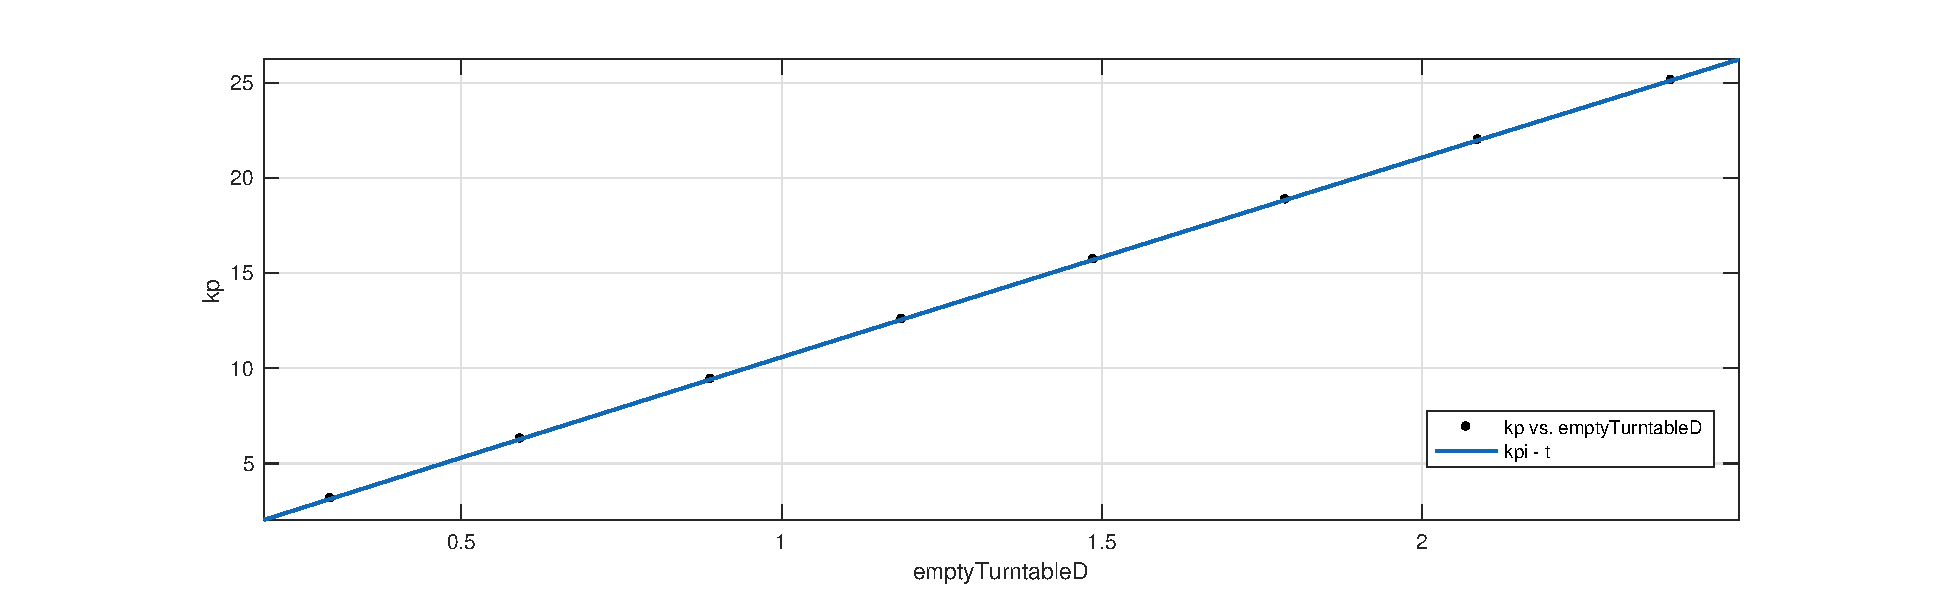
\includegraphics[width=\EFWwr]{matlab/etd}
\end{figure}

$$ \beta_1 = -0.0970 radius/s^2$$ (with 95\% confidence bounds) 

\begin{figure}[H]
\centering
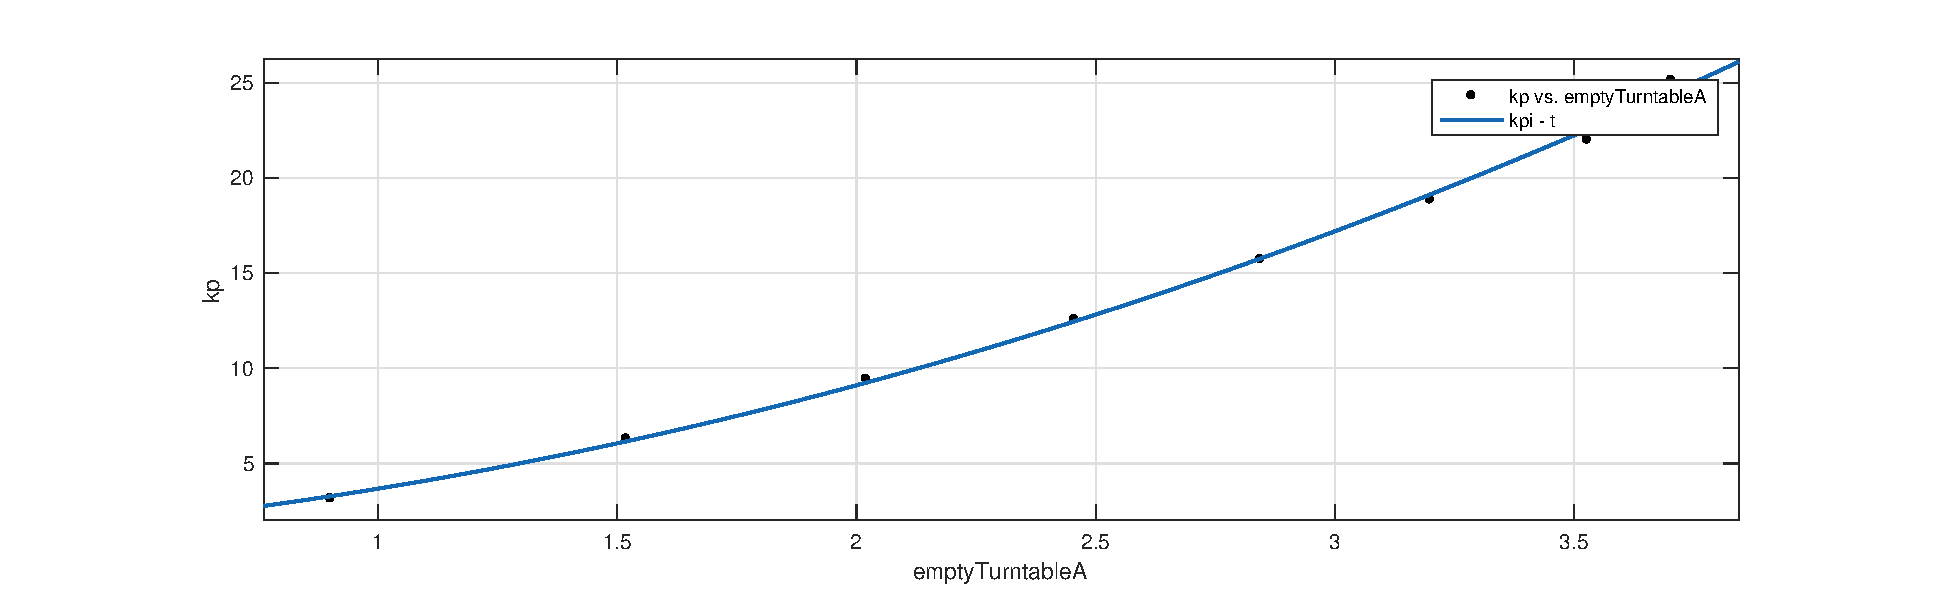
\includegraphics[width=\EFWwr]{matlab/eta}
\end{figure}

$$ \beta_2 = 2.6580 radius/s^2$$ (with 95\% confidence bounds) 

Thus,
$$ I_1 = \frac{59.1 g \times 5.0145 cm \times (9.80665 m/s^2 - 5.0145 cm \times (-0.0970) radius/s^2 )}{2.6580 radius/s^2 -(-0.0970 radius/s^2) } = 0.0105 kg\times m^2 $$

% ==================================================================
% ==================================================================
For turntable with disk,
\begin{figure}[H]
\centering
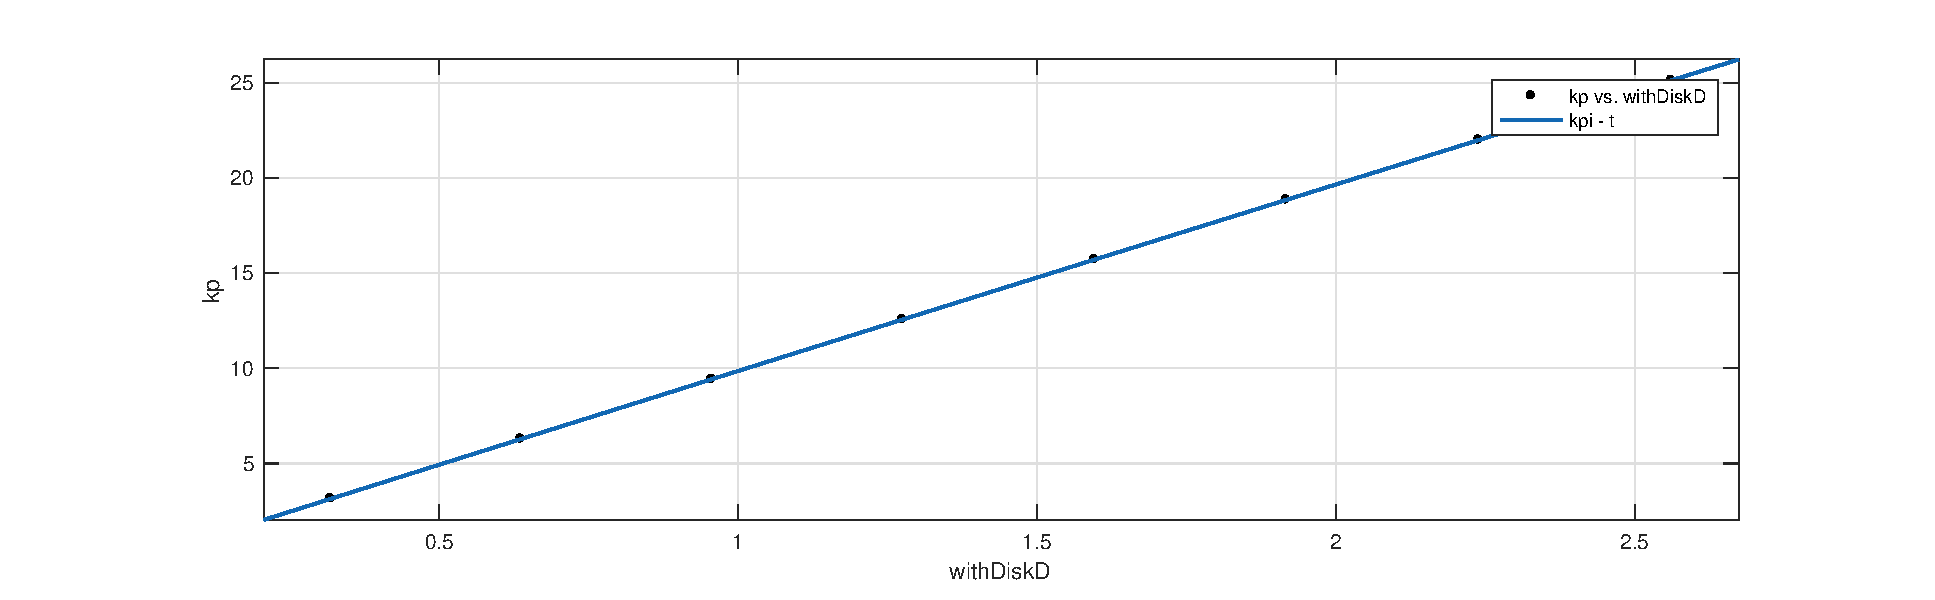
\includegraphics[width=\EFWwr]{matlab/wdd}
\end{figure}

$$ \beta_1 = -0.0668 radius/s^2$$ (with 95\% confidence bounds) 

\begin{figure}[H]
\centering
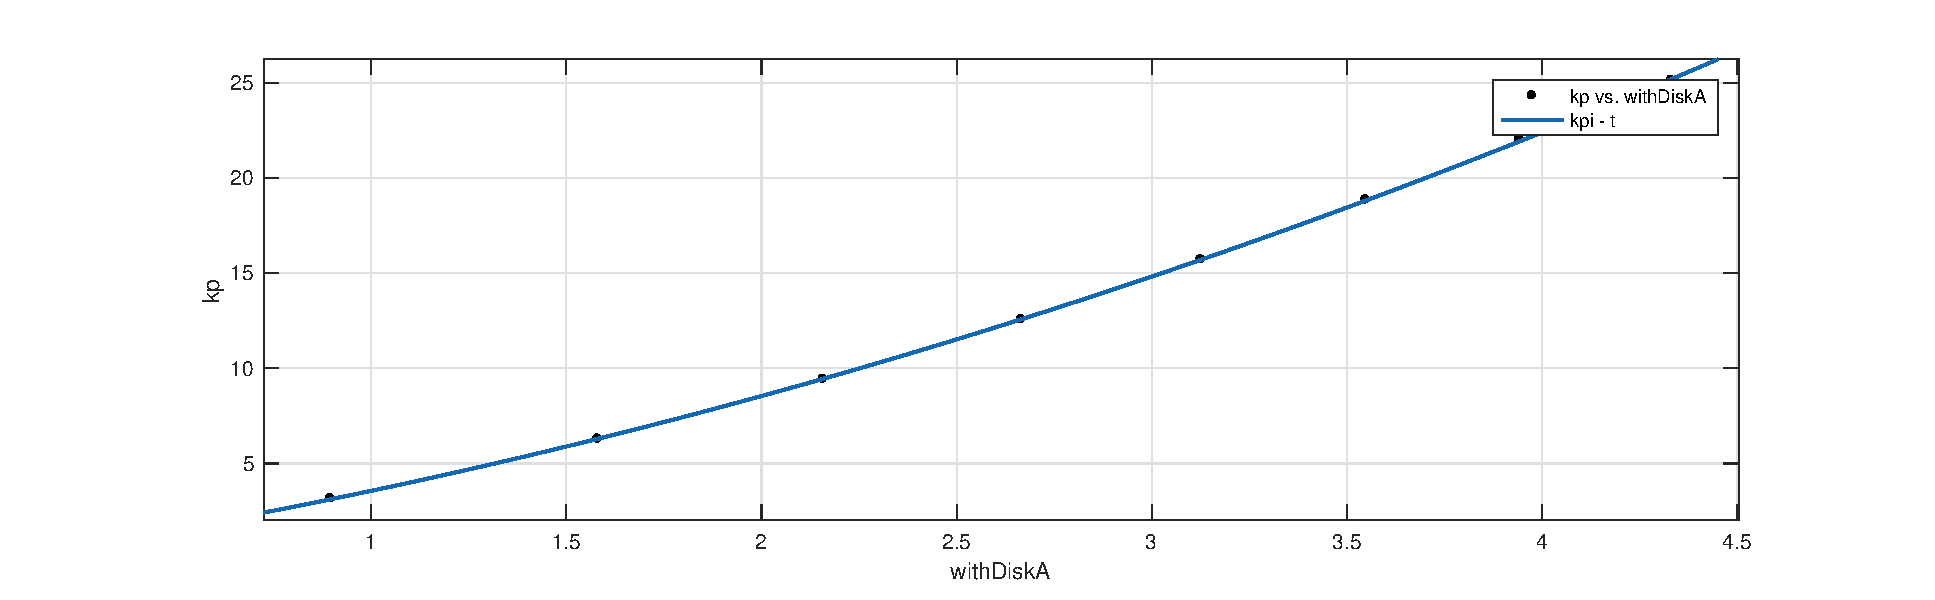
\includegraphics[width=\EFWwr]{matlab/wda}
\end{figure}

$$ \beta_2 = 1.2970 radius/s^2$$ (with 95\% confidence bounds) 

$$ I_2 = \frac{59.1 g \times 5.0145 cm \times (9.80665 m/s^2 - 5.0145 cm \times (-0.0668) radius/s^2 )}{1.2970 radius/s^2 -(-0.0668 radius/s^2) } = 0.0213 kg\times m^2 $$


% ==================================================================
% ==================================================================
For turntable with hoop,

\begin{figure}[H]
\centering
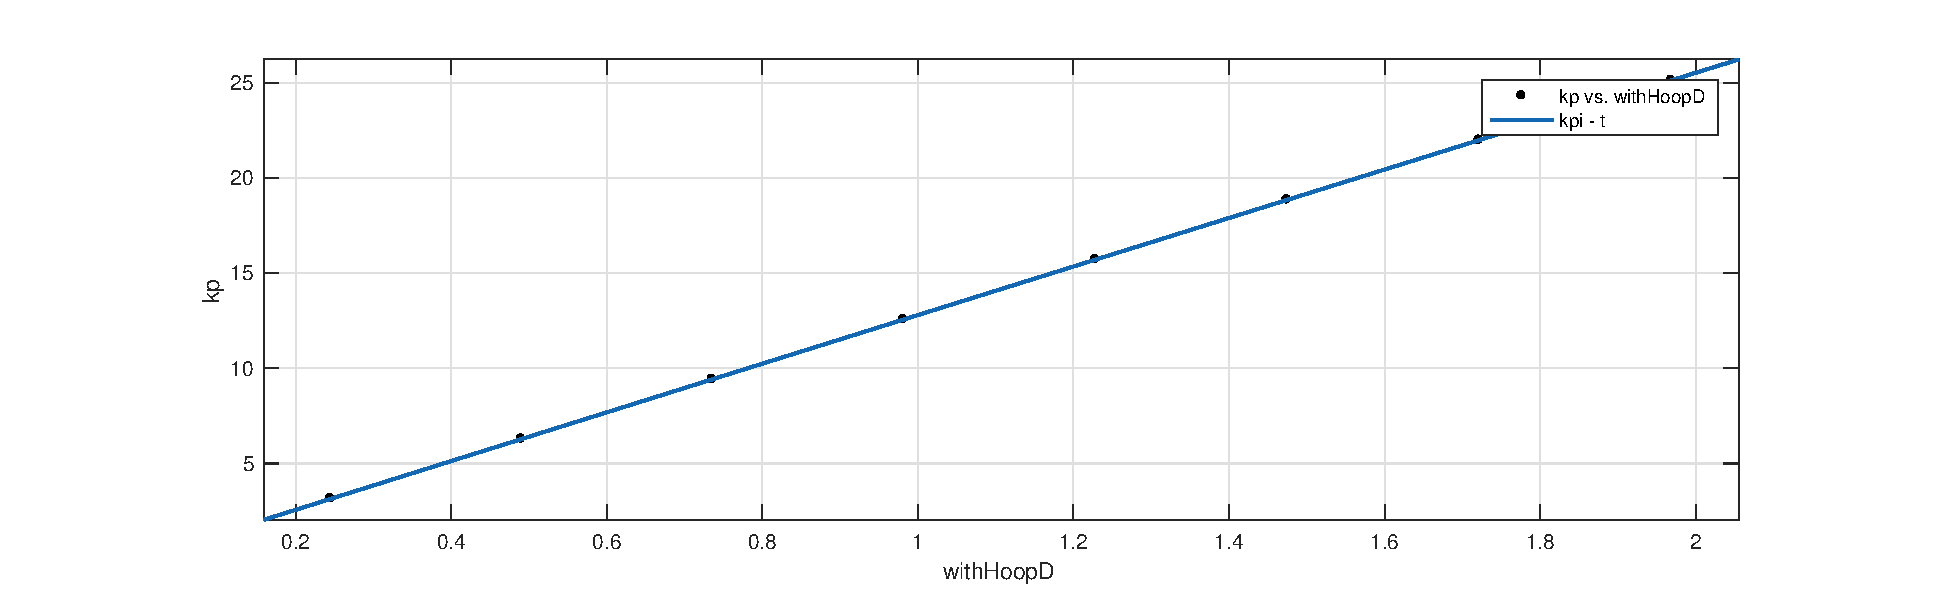
\includegraphics[width=\EFWwr]{matlab/whd}
\end{figure}

$$ \beta_1 = -0.0689 radius/s^2$$ (with 95\% confidence bounds) 

\begin{figure}[H]
\centering
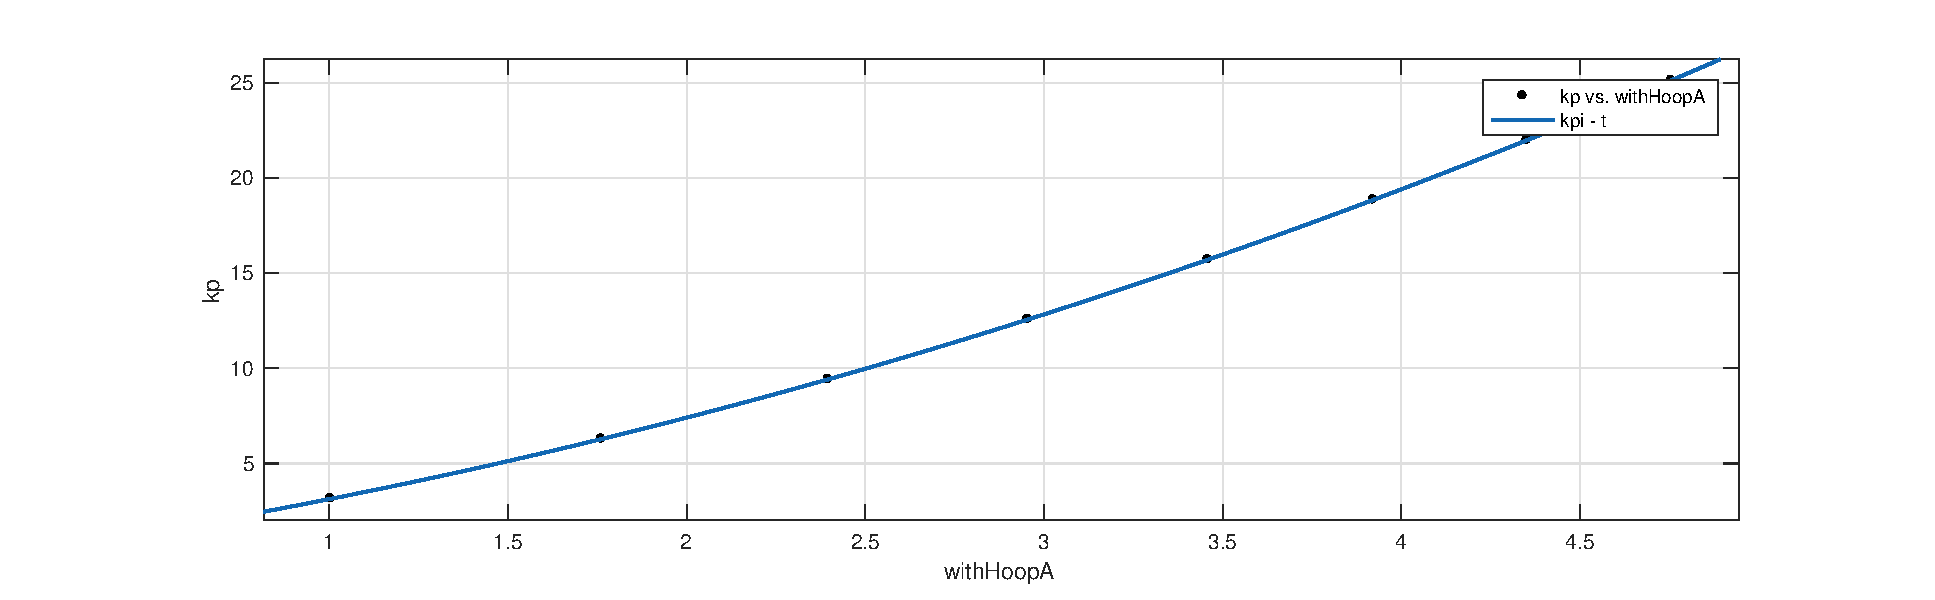
\includegraphics[width=\EFWwr]{matlab/wha}
\end{figure}

$$ \beta_2 = 1.1444 radius/s^2$$ (with 95\% confidence bounds) 


$$ I_3 = \frac{59.1 g \times 5.0145 cm \times (9.80665 m/s^2 - 5.0145 cm \times (-0.0689) radius/s^2 )}{1.1444 radius/s^2 -(-0.0689 radius/s^2) } =  0.0240 kg\times m^2 $$


% ==================================================================
% ==================================================================
For Cylinder A in hole 1, B in hole 2

\begin{figure}[H]
\centering
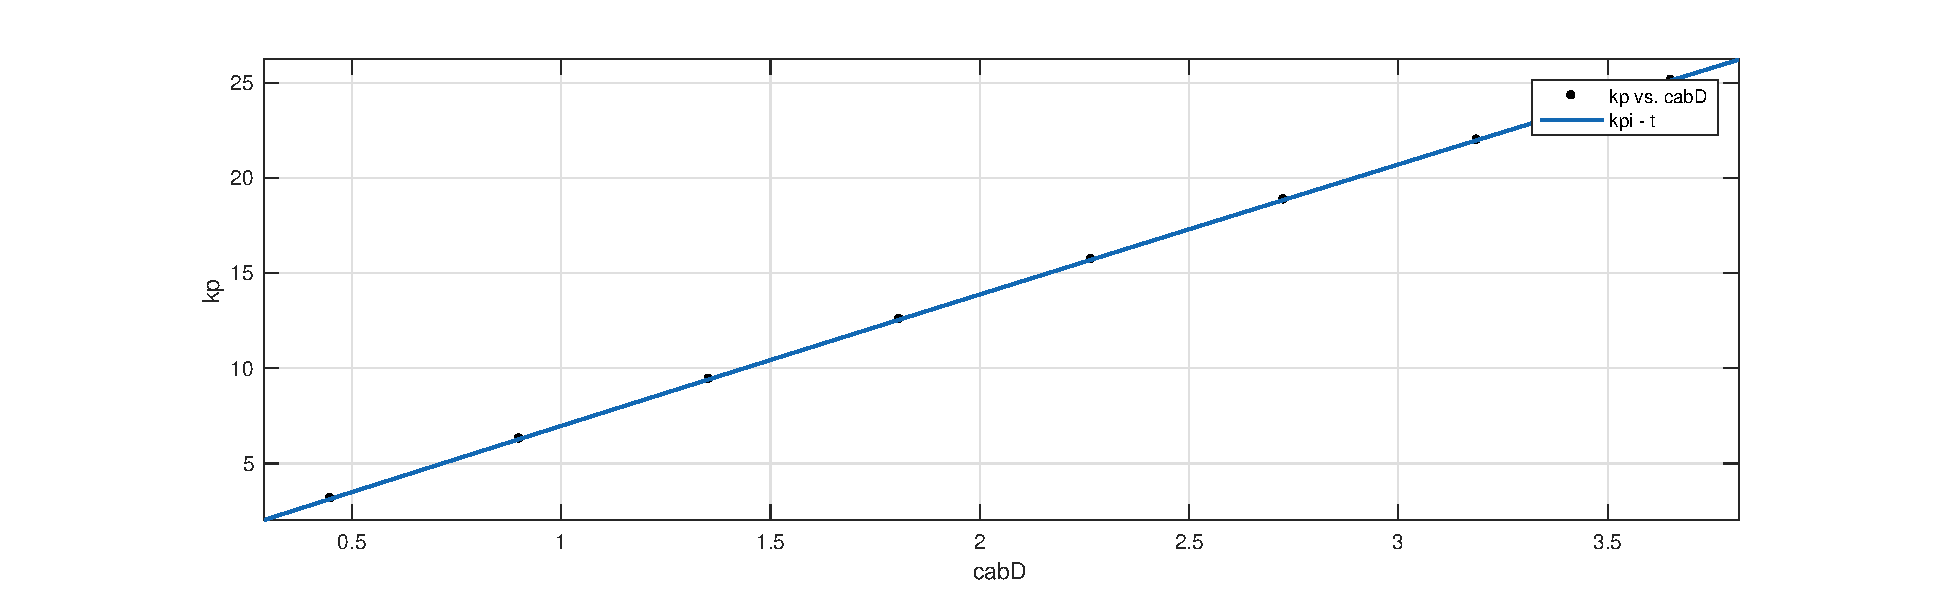
\includegraphics[width=\EFWwr]{matlab/cabd}
\end{figure}

$$ \beta_1 = -0.0710 radius/s^2$$ (with 95\% confidence bounds) 

\begin{figure}[H]
\centering
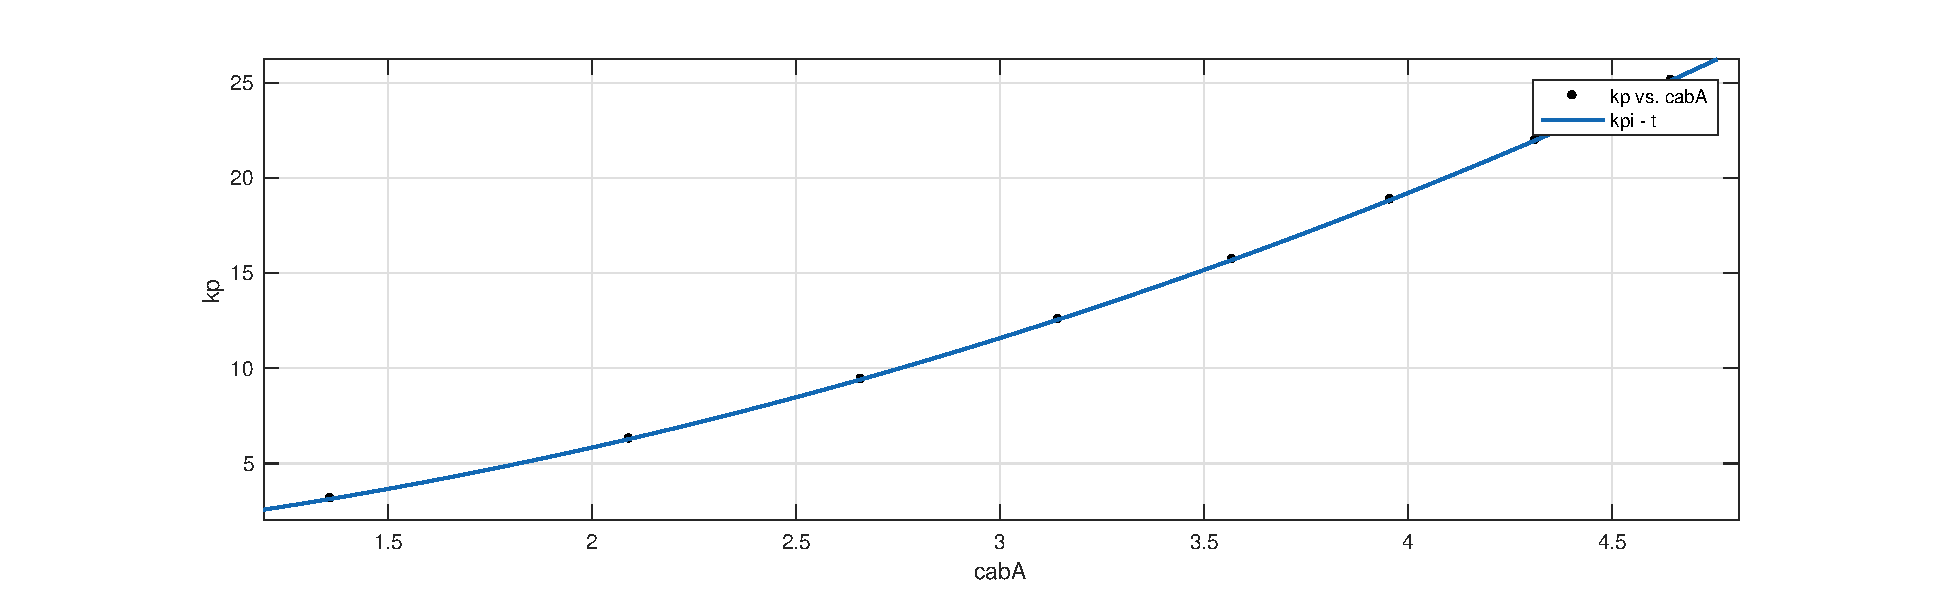
\includegraphics[width=\EFWwr]{matlab/caba}
\end{figure}

$$ \beta_2 = 1.8752 radius/s^2$$ (with 95\% confidence bounds) 


$$ I_4 = \frac{59.1 g \times 5.0145 cm \times (9.80665 m/s^2 - 5.0145 cm \times (-0.0710) radius/s^2 )}{1.8752 radius/s^2 -(-0.0710 radius/s^2) } =  0.0149 kg\times m^2 $$


% ==================================================================
% ==================================================================
For Cylinder A in hole 3, B in hole 4

\begin{figure}[H]
\centering
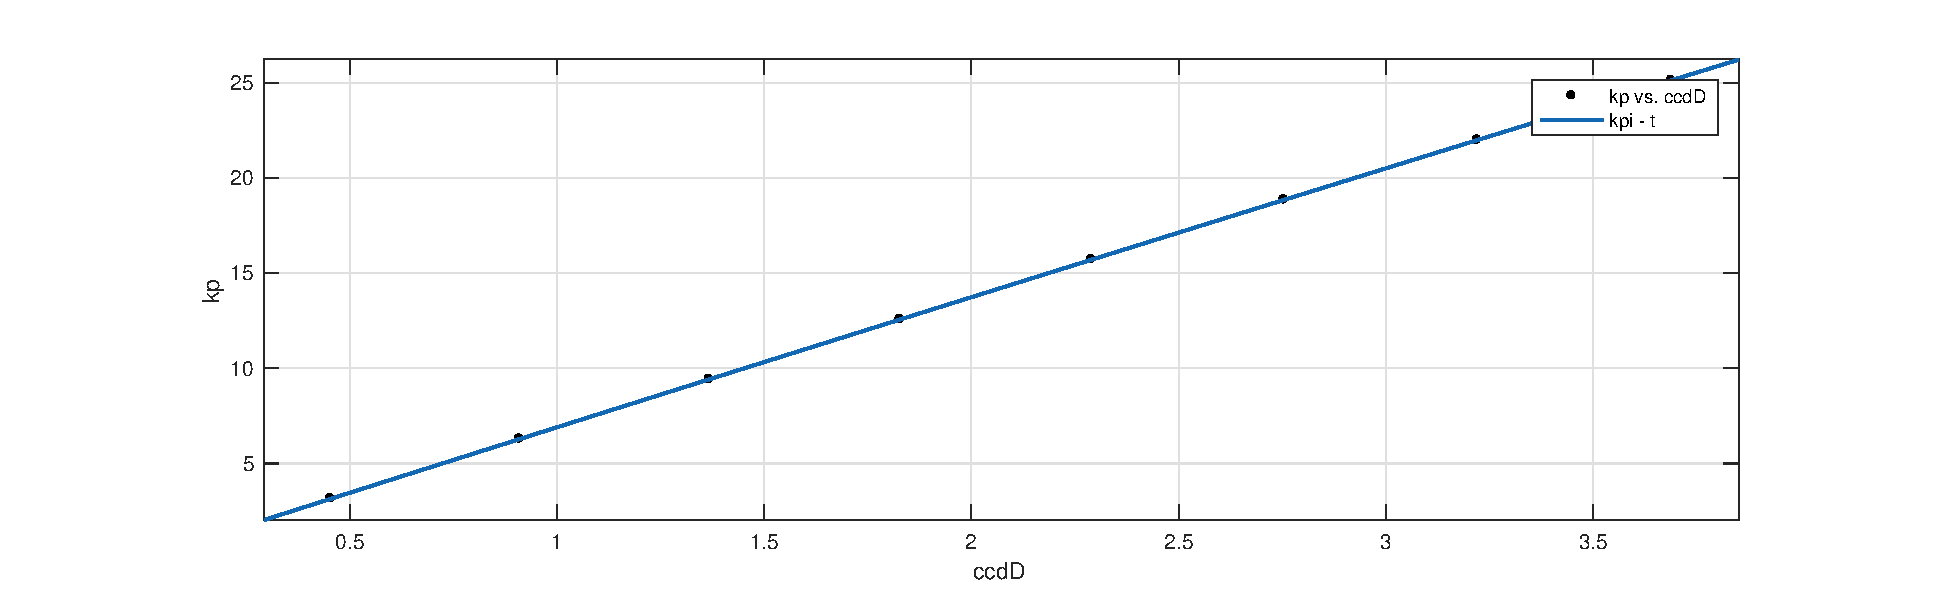
\includegraphics[width=\EFWwr]{matlab/ccdd}
\end{figure}

$$ \beta_1 = -0.0661 radius/s^2$$ (with 95\% confidence bounds) 

\begin{figure}[H]
\centering
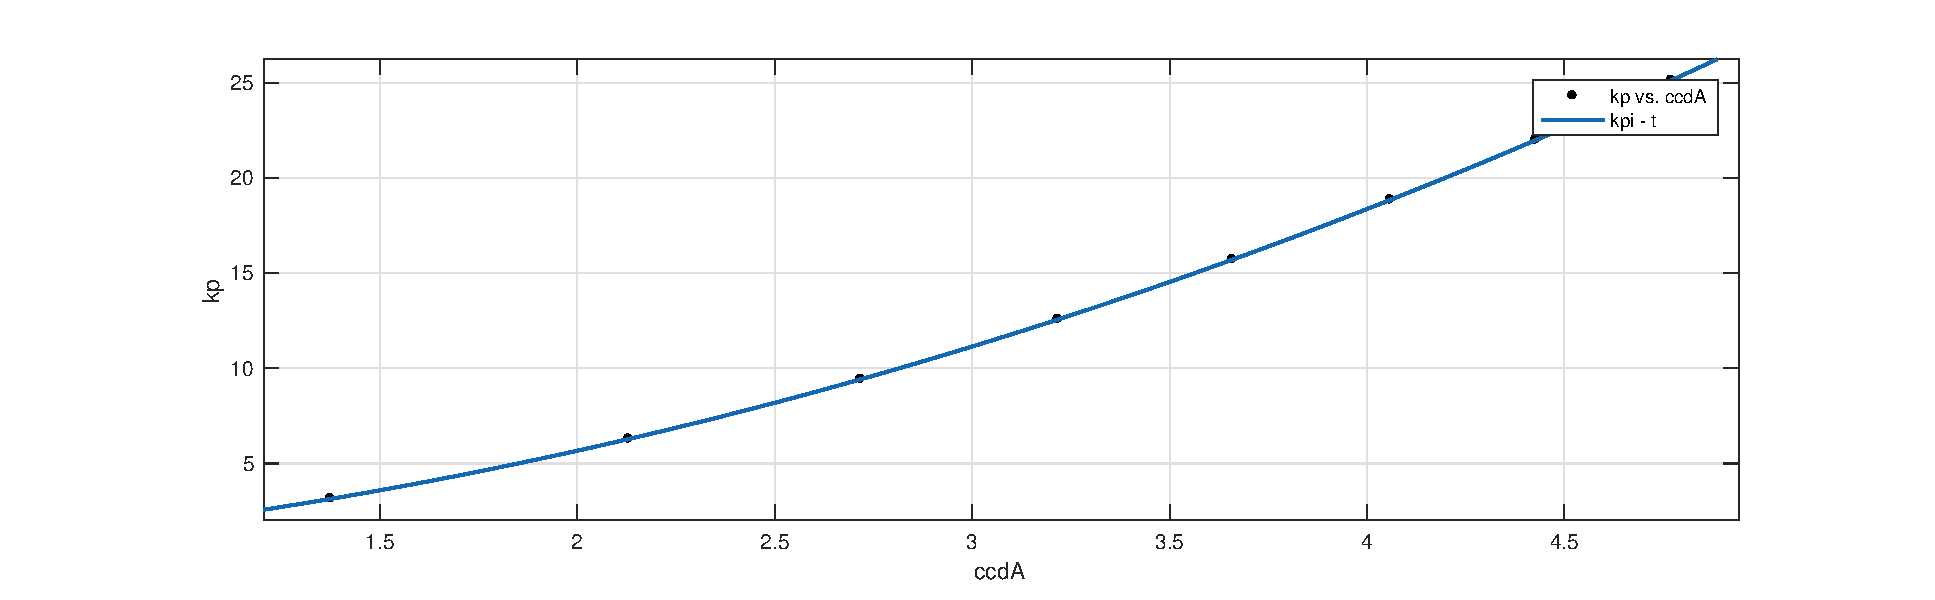
\includegraphics[width=\EFWwr]{matlab/ccda}
\end{figure}

$$ \beta_2 = 1.7496 radius/s^2$$ (with 95\% confidence bounds) 


$$ I_5 = \frac{59.1 g \times 5.0145 cm \times (9.80665 m/s^2 - 5.0145 cm \times (-0.0661) radius/s^2 )}{ 1.7496 radius/s^2 -(-0.0661 radius/s^2) } = 0.0160 kg\times m^2 $$

Thus, the moment of inertia for disk is 
$$ I_{disk} = I_2 - I_1 = 0.0213  kg\times m^2 - 0.0105 kg\times m^2 =  0.0108  kg\times m^2 $$

The moment of inertia for hoop is 
$$ I_{hoop} = I_3 - I_1 = 0.0240  kg\times m^2 - 0.0105 kg\times m^2 =  0.0135  kg\times m^2 $$

The moment of inertia for Cylinder A in hole 1 and Cylinder B in hole 2 is 
$$ I_{A1B2} = I_4 - I_1 = 0.0149  kg\times m^2 - 0.0105 kg\times m^2 =  0.0044  kg\times m^2 $$

The moment of inertia for Cylinder A in hole 3 and Cylinder B in hole 4 is 
$$ I_{A3B4} = I_5 - I_1 = 0.0160  kg\times m^2 - 0.0105 kg\times m^2 =  0.0055  kg\times m^2 $$

$$ I_{A3B4} -I_{A1B2} =0.0055  kg\times m^2 -   0.0044  kg\times m^2 = 0.0011 kg\times m^2  $$
$$ md^2 =  165.8 g \times  (4.7560 cm - 6.0120cm )^2 + 165.8 g \times  (4.7610 cm - 6.0200cm )^2  = 0.0052436 kg\times m^2 $$

Thus, the relative uncertainty is $$ \frac{ 0.0055  kg\times m^2 - 0.0052436 kg \times m^2}{0.0055  kg\times m^2} = 4.66 \% $$



\section{Measurement Uncertainty Analysis}


\subsection{Uncertainty of instruments}
For a single measurement of the mass of the experiment setup, the uncertainty of the measurement instruments are

\begin{table}[H]
  \centering
  \begin{tabularx}{\textwidth}{|X|X|X|X|}
    \hline
     & Calliper & Electronic balance & Timer\\
	 \hline
	 Resolution & 0.002cm & 0.1g & 0.0001s \\
	 \hline
	 Relative uncertainty &\multicolumn{2}{c|}{}& 0.004\% \\
	\hline
  \end{tabularx}
  \caption{Precision of the measurement instruments}
  \end{table}

\subsection{Uncertainty of Calliper Measurements}

In order to estimate type–A uncertainty of the period, the standard deviation of the average value is calculated as
$$  s_d = \sqrt{\frac{1}{n-1}\sum_{i=1}^{n}(d_i - \bar{d})^2 }  $$

Thus, the standard deviation of the average value is calculated and shown below

\begin{table}[H]
  \centering
  \begin{tabularx}{\textwidth}{|p{6cm}|X|}
    \hline
    Object & The standard deviation\\
    \hline
    Disk $[cm]$& 0.0020 \\
    Hoop 1 $[cm]$& 1.1003 \\
    Hoop 2 $[cm]$& 1.1017 \\
    Cylinder A $[cm]$& 0 \\
    Cylinder B $[cm]$& 0 \\
    Cone pulley $[cm]$& 0.0075 \\
    \hline
  \end{tabularx}
  \caption{The standard deviation}
  \end{table}


The uncertainty of Timer is $\pm 0.0001s $ and $\pm 0.004\%$

From the equation to calculate the moment of inertia,
$$ I_1=\frac{mR(g-R\beta_2)}{\beta_2-\beta_1} $$
$$ u_F = \sqrt{(\frac{\partial I}{\partial m})^2(u_m)^2 +   (\frac{\partial I}{\partial R})^2(u_R)^2+(\frac{\partial I}{\partial \beta_1 })^2(u_{\beta_1})^2+ (\frac{\partial I}{\partial \beta_2})^2(u_{\beta_2})^2   }$$

$$\frac{\partial I}{\partial m} = \frac{R\left(g-\beta _2 R\right)}{\beta _2-\beta _1} $$
$$\frac{\partial I}{\partial R} = -\frac{\beta _2 m R'\left(g-\beta _2 R\right)}{\beta _2-\beta _1} $$
$$\frac{\partial I}{\partial \beta_1} = \frac{m R\left(g-\beta _2 R\right)}{\left(\beta _2-\beta _1\right){}^2} $$
$$\frac{\partial I}{\partial \beta_2} = -\frac{m R R'\left(g-\beta _2 R\right)}{\beta _2-\beta _1}-\frac{m R\left(g-\beta _2 R\right)}{\left(\beta _2-\beta _1\right){}^2} $$


$$ u_m = 0.1 g $$
$$ u_R = 0.0075 cm $$
$$ u_{\beta_1} = \sqrt{(0.0001 s)^2+(0.0001 \times 95 \% )^2} =0.000137931 $$
$$ u_{\beta_1} = \sqrt{(0.0001 s)^2+(0.0001 \times 95 \% )^2} =0.000137931 $$

Thus, 
$$u_{rF} =  0.4\%$$


\section{Conclusions and Discussion}

In the experiment, the moment of inertia is found by measuring the angular acceleration of the turntable in different cases. 

By plotting and fitting the relation between $k\pi$ and $ t $, we found the $\beta$ for each situation of the instrument.
For we used MATLAB to do the fitting work, the uncertainty of the fitting curve can be easily seen as $\pm 5\%$.

By comparing the calculated value of the difference of $I_A$ and $I_B$, we can use the experiment to judge whether the parallel axis theorem holds.

The calculated value of $I$ is $md^2 =  165.8 g \times  (4.7560 cm - 6.0120cm )^2 + 165.8 g \times  (4.7610 cm - 6.0200cm )^2  = 0.0052436 kg\times m^2 $ and the value derived from the experiment is $ I_{A3B4} -I_{A1B2} =0.0055  kg\times m^2 -   0.0044  kg\times m^2 = 0.0011 kg\times m^2 $.
The relative uncertainty is $$ \frac{ 0.0055  kg\times m^2 - 0.0052436 kg \times m^2}{0.0055  kg\times m^2} = 4.66 \% $$

Thus, the parallel axis theorem holds very well.

The g

\section{Reference}

\begin{enumerate}
\item  The international system of units (SI) (PDF) (2008 ed.). United States Department of Commerce, NIST Special Publication 330. pp. 29 \& 57.
\end{enumerate}

\section{Data Sheet}

% data sheet

\end{document}